\documentclass{article}

%%%%%%%%%%%%%%%%%%%%%%%%%%%%%%%%%%%%%
%%% AUTHOR PACKAGES %%%%%%%%%%%%%%%%%
%%%%%%%%%%%%%%%%%%%%%%%%%%%%%%%%%%%%%

\usepackage{amsmath}
\usepackage{amssymb}
\usepackage{nicefrac}
\usepackage{tikz}
\usetikzlibrary{arrows.meta}
\usepackage{subcaption}
\DeclareMathOperator{\ext}{ext}
\DeclareMathOperator{\conv}{conv}
\DeclareMathOperator{\dist}{dist}
\DeclareMathOperator{\Lim}{Lim^1}
\DeclareMathOperator{\diag}{diag}
\DeclareMathOperator{\trace}{Tr}
\DeclareMathOperator{\spans}{span}
\DeclareMathOperator{\ind}{ind}
\DeclareMathOperator{\spec}{\sigma}
\newcommand{\essspec}{\spec_{\mathrm{ess}}}
\newcommand{\Hil}{\ensuremath{\mathcal{H}}}
\newcommand{\vmid}{\,\middle\vert\,}
\renewcommand{\epsilon}{\varepsilon}
\renewcommand{\emptyset}{\varnothing}

%%%%%%%%%%%%%%%%%%%%%%%%%%%%%%%%%%%%%
%%% POSTER PACKAGES; LOAD LAST %%%%%%
%%%%%%%%%%%%%%%%%%%%%%%%%%%%%%%%%%%%%

\usepackage{siue-poster-settings}
\usepackage{harper-subdued}


\begin{document}

%%%%%%%%%%%%%%%%%%%%%%%%%%%%%%%%%%%%% 
%%% FONTS AND BASIC COLOR PALETTE %%%
%%%%%%%%%%%%%%%%%%%%%%%%%%%%%%%%%%%%%

\setmainfont{Linux Libertine}
\setsansfont{DejaVu Sans}
\LARGE\sffamily
\colorpalette{siuesubdued}

%%%%%%%%%%%%%%%%%%%%%%%%%%%%%%%%%%%%%
%%% TITLE AND AUTHOR INFORMATION %%%%
%%%%%%%%%%%%%%%%%%%%%%%%%%%%%%%%%%%%%

\title{Diagonals of Finite Spectrum Normal \\ Operators and Essential Codimension}
\author{Jireh Loreaux}
\maketitle

%%%%%%%%%%%%%%%%%%%%%%%%%%%%%%%%%%%%%
%%% SIUE LOGO PLACEMENT %%%%%%%%%%%%%
%%%%%%%%%%%%%%%%%%%%%%%%%%%%%%%%%%%%%

\begin{staticcontents*}{logo}
  \flushright{\includegraphics[height=0.66in]{dl_siue_br.pdf}}
\end{staticcontents*}

%%%%%%%%%%%%%%%%%%%%%%%%%%%%%%%%%%%%%
%%% BEGIN FLOW BOXES %%%%%%%%%%%%%%%%
%%%%%%%%%%%%%%%%%%%%%%%%%%%%%%%%%%%%%

\section*{Introduction}

In his seminal paper Kadison proved the following characterization of diagonals of projections which he referred to as the Carpenter's and Pythagorean Theorems.

\begin{thmcustom}{Kadison's Theorem}
  A sequence $(d_n)_{n=1}^{\infty}$ is the diagonal of a projection if and only if it takes values in the unit interval and the quantities
  \begin{equation*}
    a := \sum_{d_n < \nicefrac{1}{2}} d_n \quad\text{and}\quad b := \sum_{d_n \ge \nicefrac{1}{2}} (1-d_n)
  \end{equation*}
  satisfy one of the mutually exclusive conditions
  \begin{enumerate}
  \item $a+b = \infty$;
  \item $a+b < \infty$ and $a-b \in \mathbb{Z}$.
  \end{enumerate}
\end{thmcustom}

Arveson soon recognized this integer as the index of a Fredholm operator and referred to it as an ``index obstruction'' to an arbitrary sequence being a diagonal of a projection.
Arveson extended this index obstruction to certain normal operators.

\begin{definition}
  Given a $X \subset \mathbb{C}$, define the sequences which \strengthen{accumulate summably} at $X$ by
  \begin{equation*}
    \Lim (X) := \left\{ (d_n) \in \ell^{\infty} \mid \sum_{n=1}^{\infty} \dist(d_n,X) < \infty \right\}.
  \end{equation*}
\end{definition}

\begin{thmcustom}{Arveson's Index Obstruction}
  Let $N := \sum_{k=1}^m \lambda_k P_k$ be a normal operator with finite spectrum $X = \{\lambda_1,\ldots,\lambda_m\}$ coincident with its essential spectrum whose elements are the vertices of a convex polygon in $\mathbb{C}$, and let $(d_n)$ be a diagonal of $N$.
  If $(d_n) \in \Lim (X)$, then for any choice $x_n \in X$ for which $(d_n-x_n)$ is absolutely summable, there exist \strengthen{integers} $c_1,\ldots,c_m$ which sum to zero for which
  \begin{equation*}
    \sum_{n=1}^{\infty} (d_n-x_n) = \sum_{k=1}^m c_k \lambda_k.
  \end{equation*}
\end{thmcustom}

\framebreak

\section*{Main Results}

Our first result provides an operator-theoretic condition that is equivalent to the hypotheses of Arveson's Theorem.

\begin{theorem}
  Let $N$ be a normal operator with finite spectrum and diagonal $(d_n)$, and let $X$ be the vertices of the convex hull of the essential spectrum.
  Then $(d_n) \in \Lim(X)$ if and only if $\essspec(N) = X$ and $N$ is diagonalizable by a unitary which is a Hilbert--Schmidt perturbation of the identity.
\end{theorem}

Arveson's Theorem may then be restated as the following.

\begin{thmcustom}{Arveson Reformulated}
  Let $N$ be a normal operator with $\spec(N) = \essspec(N)$ that is diagonalizable by a unitary which is a Hilbert--Schmidt perturbation of the identity.
  Then there is a diagonal operator $N'$ with $\spec(N') \subseteq \spec(N)$ for which $E(N'-N)$ is trace-class, and for any such operator, $\trace(E(N'-N)) \in K_{\spec(N)}$.
\end{thmcustom}

It turns out that this version of Arveson's Theorem is a corollary of a far more general result.

\begin{theorem}
  Suppose $N$ is a normal operator.
  There is a diagonal masa such that for every unitary $U = I + K$ with $K$ Hilbert--Schmidt, then $E(UNU^{*}-N)$ is trace-class and has trace zero.
  Moreover, if $N$ is diagonalizable, any masa containing $N$ suffices.
\end{theorem}

\begin{remark}
  In the proof of the above theorem, normality is used only to write $N$ as a Hilbert--Schmidt perturbation of a diagonal operator via Voiculescu's extension of the Weyl--von Neumann--Berg theorem.
  Hence, there is a slightly more general but less interesting result for such operators.
\end{remark}

\framebreak

\section*{Examples}

\vfill

\begin{figure}[h!]
  \begin{subfigure}{0.5\linewidth}
  \centering
  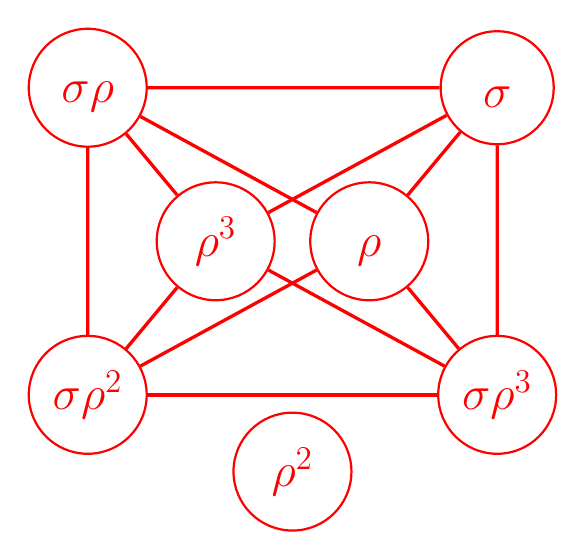
\begin{tikzpicture}[scale=1.3]
    \begin{scope}[every node/.style={circle,thick,draw,red,font=\LARGE,text width={1cm},text height={0.5cm},align=center}]
      \node (sr) at (-2,1.5) {$\sigma\rho$};
      \node (s) at (2,1.5) {$\sigma$};
      \node (r3) at (-0.75,0) {$\rho^3$};
      \node (r) at (0.75,0) {$\rho$};
      \node (sr2) at (-2,-1.5) {$\sigma\rho^2$};
      \node (sr3) at (2,-1.5) {$\sigma\rho^3$};
      \node (r2) at (0,-2.25) {$\rho^2$};
    \end{scope}
    \begin{scope}[
      every edge/.style={draw=red,very thick}]
      \path (sr) edge (s);
      \path (sr) edge (sr2);
      \path (sr) edge (r3);
      \path (sr) edge (r);
      \path (s) edge (r3);
      \path (s) edge (r);
      \path (s) edge (sr3);
      \path (sr2) edge (r3);
      \path (sr2) edge (r);
      \path (sr2) edge (sr3);
      \path (sr3) edge (r3);
      \path (sr3) edge (r); 
    \end{scope}
  \end{tikzpicture}
  \caption*{\LARGE Generating graph $\Gamma(D_8)$}
\end{subfigure}%
\begin{subfigure}{0.5\linewidth}
  \centering
  \includegraphics[width=0.75\linewidth]{F2_Cayley_Graph.png}
  \caption*{\LARGE Cayley graph of $F_2$}
\end{subfigure}
\end{figure}

\vfill

\section*{Key Tools}

An essential ingredient in the arguments we present is \emph{essential codimension} due to Brown--Douglas--Fillmore.

\begin{definition}
  Given a pair of projections $P,Q$ whose difference is compact, the \strengthen{essential codimension} of $P$ in $Q$, denoted $[P:Q]$, is the integer defined by
  \begin{equation*}
    [P:Q] :=
    \begin{cases}
      \trace P-\trace Q & \text{if}\ \trace P,\trace Q < \infty, \\[1em]
      \ind(V^{*}W) & \parbox[c][3em]{0.55\textwidth}{if $\trace(P) = \trace(Q) = \infty$, where \\
        $W^{*}W = V^{*}V = I, WW^{*} = P, VV^{*} = Q$.} \\[0.4em]
    \end{cases}
  \end{equation*}
\end{definition}

We also used a recent, more detailed version of Kadison's theorem.

\begin{theorem}
  Suppose $P,Q$ are projections. Then $P-Q$ is Hilbert--Schmidt if and only if in some (equivalently, every) orthonormal basis $\{e_n\}_{n=1}^{\infty}$ which diagonalizes $Q$, the diagonal $(d_n)$ of $P$ satisfies $a+b < \infty$, where
  \begin{equation*}
    a := \sum_{e_n \in Q^{\perp}\Hil} d_n \quad\text{and}\quad b := \sum_{e_n \in Q\Hil} (1-d_n).
  \end{equation*}
  Moreover, in this case $a-b = [P:Q]$.
\end{theorem}

The final piece in the puzzle is the following link between \strengthen{restricted diagonalization} and essential codimension.

\begin{proposition}
  If $P,Q$ are projections, then $Q = UPU^{*}$ for some unitary $U = I+K$ with $K \in \mathcal{J}$ if and only if $P-Q \in \mathcal{J}$ and $[P:Q] = 0$.
\end{proposition}

%%%%%%%%%%%%%%%%%%%%%%%%%%%%%%%%%%%%%
%%% END FLOW BOXES %%%%%%%%%%%%%%%%%%
%%%%%%%%%%%%%%%%%%%%%%%%%%%%%%%%%%%%%


\end{document}
%%% Local Variables:
%%% mode: latex
%%% TeX-master: t
%%% TeX-engine: luatex
%%% End:
